%preamble
\documentclass[letterpaper]{article}
\synctex=1
\usepackage{graphicx}
\graphicspath{ {images/} }

\usepackage{lipsum}
\usepackage{float}
% \bibliographystyle{IEEEtran}
% \bibliographystyle{ieeetr}

\usepackage{amssymb}

\usepackage{siunitx}

\usepackage{multirow}
% for merging table cells I think

\usepackage{fancyhdr} %header
\fancyhf{}
\fancyhead[R]{Arun Woosaree XXXXXXX}
\renewcommand\headrulewidth{0pt}
\fancyfoot[C]{\thepage}
\renewcommand\footrulewidth{0pt}
\pagestyle{fancy}

% make subsection use letters
\renewcommand{\thesubsection}{\thesection.\alph{subsection}}


\usepackage{amsthm}
\newtheorem*{clt}{Central Limit Theorem}

%actual document
\begin{document}

% \maketitle %insert titlepage here
\begin{titlepage}
 \begin{center}
  \vspace*{1cm}
  \Huge
  Stat 235
  \vspace{1cm}
  
  Lab 3
  \vspace{1cm}
  
  WOOSAREE, Arun
  \vspace{1cm}
  
  \Huge
  Lab EL12
  \vspace{1cm}
  
  TA: Jessa Marley
  \vspace{1cm}
  
  \today
  \vfill
 \end{center}
\end{titlepage}

\section{}%1
% Use Poisson probabilities sheet.
% How does change in lambda affect shape of graph?
% How does the increase affect the quality/number of flaws?
As $\lambda$ increases, the distribution shifts to the right, since $\lambda$ is
the mean value of the distribution. We also see that as this distribution shifts
to the right, the curve flattens as a result of the mean probability decreasing
while the spread increases (Since the total area under this distribution is 1).
Since Poisson distributions measure the number of successes in an interval, and
in this case a ``success'' is a flaw in a plastic panel, we can clearly see that
for manufacturing processes with higher $\lambda$, the variability of the panels
produced increases. This means that we will see slightly more panels with flaws,
slightly more panels with less flaws, and less panels with the expected
($\lambda$) number of flaws.

\section{}%2

\subsection{}%2a
% Use Poisson probabilities sheet
% What value should x have?
\label{2a}
Assuming $\lambda=0.5$, the probability that there are no flaws in a randomly
selected panel is $P(X=0)$. Using the \textit{Poisson Probabilities} worksheet,
we find this number to be $0.6065$, or $60.65\%$ of the panels are in perfect
condition

\subsection{}%2b
\label{2b}
% Use Poisson probabilities sheet
% What probability should go in the distribution? Choose carefully
The percentage of panels with 2 or more flaws can be found as shown below:
$$P(X\geq2)=1-P(X<2) = 1-P(X\leq1)$$
Using the \textit{Poisson Probabilities} worksheet,
we find $P(X\leq1)=0.9098$, so
$$P(X\geq2) = 1-0.9098 = 0.0902 $$
So, $9.02\%$ of the panels would need to be scrapped.


\subsection{}%2c
\label{2c}
% Use Poisson probabilities sheet
% MAYBE there's something useful in part b .. think of them as 10 independent events
% ex: how do we find trhe probability of getting 2 heads in a row for a coin toss?
% 1/2 * 1/2 = 1/4
From \ref{2b}, we know the probability of a single panel not being defective is $P(X\leq1)=0.9098$.
For ten panels, $$ P(X\leq1)^{10} = 0.9098^{10} = 0.38856110447...$$
Therefore, the probability that a random sample of 10 panels not containing
a defective panel is approximately $0.389$.


\section{}%3
From in-class notes, the Central Limit Theorem states the following:
\begin{clt}
 When $n$ is sufficiently large, the sampling distibution of $\bar{x}$ is well
 approximated by a normal curve, even when the population distibution is not
 itself normal. The Central Limit Theorem can safely be applied if $n$ is at
 least 30.
\end{clt}

Note: For Question 3, $\lambda=0.5$
\subsection{}%3a
% Use the normal probabilities sheet
% Why can't we assume that the distribution of the sample mean is normal?
% (Think sample size, central limit theorem)
% Find the variance and mean to get probability
\label{3a}
Referring to the Central Limit Theorem as defined above, we cannot safely assume
that the sampling distribution of the average number of flaws in a random sample
of 10 panels follows approximately a normal distribution. The Central Limit
Theorem states that it can only be safely applied when the sample size is
greater than or equal to 30.

If we were to assume that the Central Limit Theorem does apply, however, the
probability that the average number of flaws in a random sample of 10 panels
does not exceed 0.3 is found as follows:

$$\sigma^2 = \lambda \Rightarrow
 \sigma = \sqrt{\lambda} = \sqrt{0.5} = \frac{1}{\sqrt{2}} $$

$$\Rightarrow \sigma_{\bar{x}} = \frac{\sigma}{\sqrt{n}} =
 \frac{1/\sqrt{2}}{\sqrt{10}} = \frac{1}{\sqrt{20}} \approx 0.2236 $$

Plugging in $\lambda$, and $\sigma_{\bar{x}}$ into the \textit{Normal Probabilities Sheet},
we find that $P(X \leq 0.30) = 0.1855$.

\subsection{}%3b
% Use the normal probabilities sheet
% Why can't we assume that the distribution of the sample mean is normal?
% (Think sample size, central limit theorem)
% Find the variance and mean to get probability
We can safely assume that the sampling distribution of the average number of
flaws in a random sample of 30 panels follows approximately a normal
distribution, because a sample size of 30 satisfies the condition in the Central
Limit Theorem which requires a sample size greater than or equal to 30.

Assuming that the Central Limit Theorem does applies, the
probability that the average number of flaws in a random sample of 30 panels
does not exceed 0.3 is found as follows:

$$\sigma_{\bar{x}} = \frac{\sigma}{\sqrt{n}} =
 \frac{1/\sqrt{2}}{\sqrt{30}} = \frac{1}{\sqrt{60}} \approx 0.129 $$

Plugging in $\lambda$, and $\sigma_{\bar{x}}$ into the \textit{Normal Probabilities Sheet},
we find that $P(X \leq 0.30) = 0.0607$.

\section{CHECK TO SEE IF YOUR RANDOM NUMBERS ARE GOOD}%4
% DO NOT CHANGE THE FORMULAS IN THE ROWS AVERAGE, COUNT, AVERAGE summary statistics

\subsection{}%4a
% Use Simulation sheet in cells B9:BI18
% Random number generation -> #variables=60 -> randomvars=10
% -> distribution=Poisson -> seed=100 -> lambda=COUNTIF()
Using the built in COUNTIF function, we find the number of perfect panels to be
362. So, the percentage of perfect panels can be found as follows:
$$\frac{362}{600}\times 100 = 60.333333333...\%$$
Therefore, about $60.33\%$ of the panels are in perfect condition. Compared with
the value obtained in \ref{2a} ($60.65\%$), it is pretty close. We expect these
values to be close, because the random data is based on the same distribution as
in \ref{2a}. However, it would be unrealistic to expect that these two values
are exactly the same, since the value obtained in \ref{2a} is a theoretical
value for an infinite number of trials, while the number obtained here is from
random data representing a finite number of plastic panels.


\subsection{}%4b
% count will be in row 42 if you generated the data correctly
Using the built in COUNTIF function, we find the number of samples with non
defective panels to be 23 So, the percentage of non defective panels can be
found as follows:
$$\frac{23}{60}\times 100 = 38.333333333\%$$
Therefore, about $38.33\%$ of the panels are not defective. Compared with the
value obtained in \ref{2c} ($38.86\%$), it is pretty close. We expect these
values to be close, because the random data is based on the same distribution as
in \ref{2c}. However, it would be unrealistic to expect that these two values
are exactly the same, due to the randomness of the generated data. Also, the
value obtained in \ref{2c} is a theoretical value for a sample of 10 from an
infinite number of panels, while we are obtaining samples from 600 randomly
generated panels.

\subsection{}%4c
% Don't over analyze, use squint test
% What's going on between 0.3 and 0.7?

\begin{figure}[H]
 \centering
 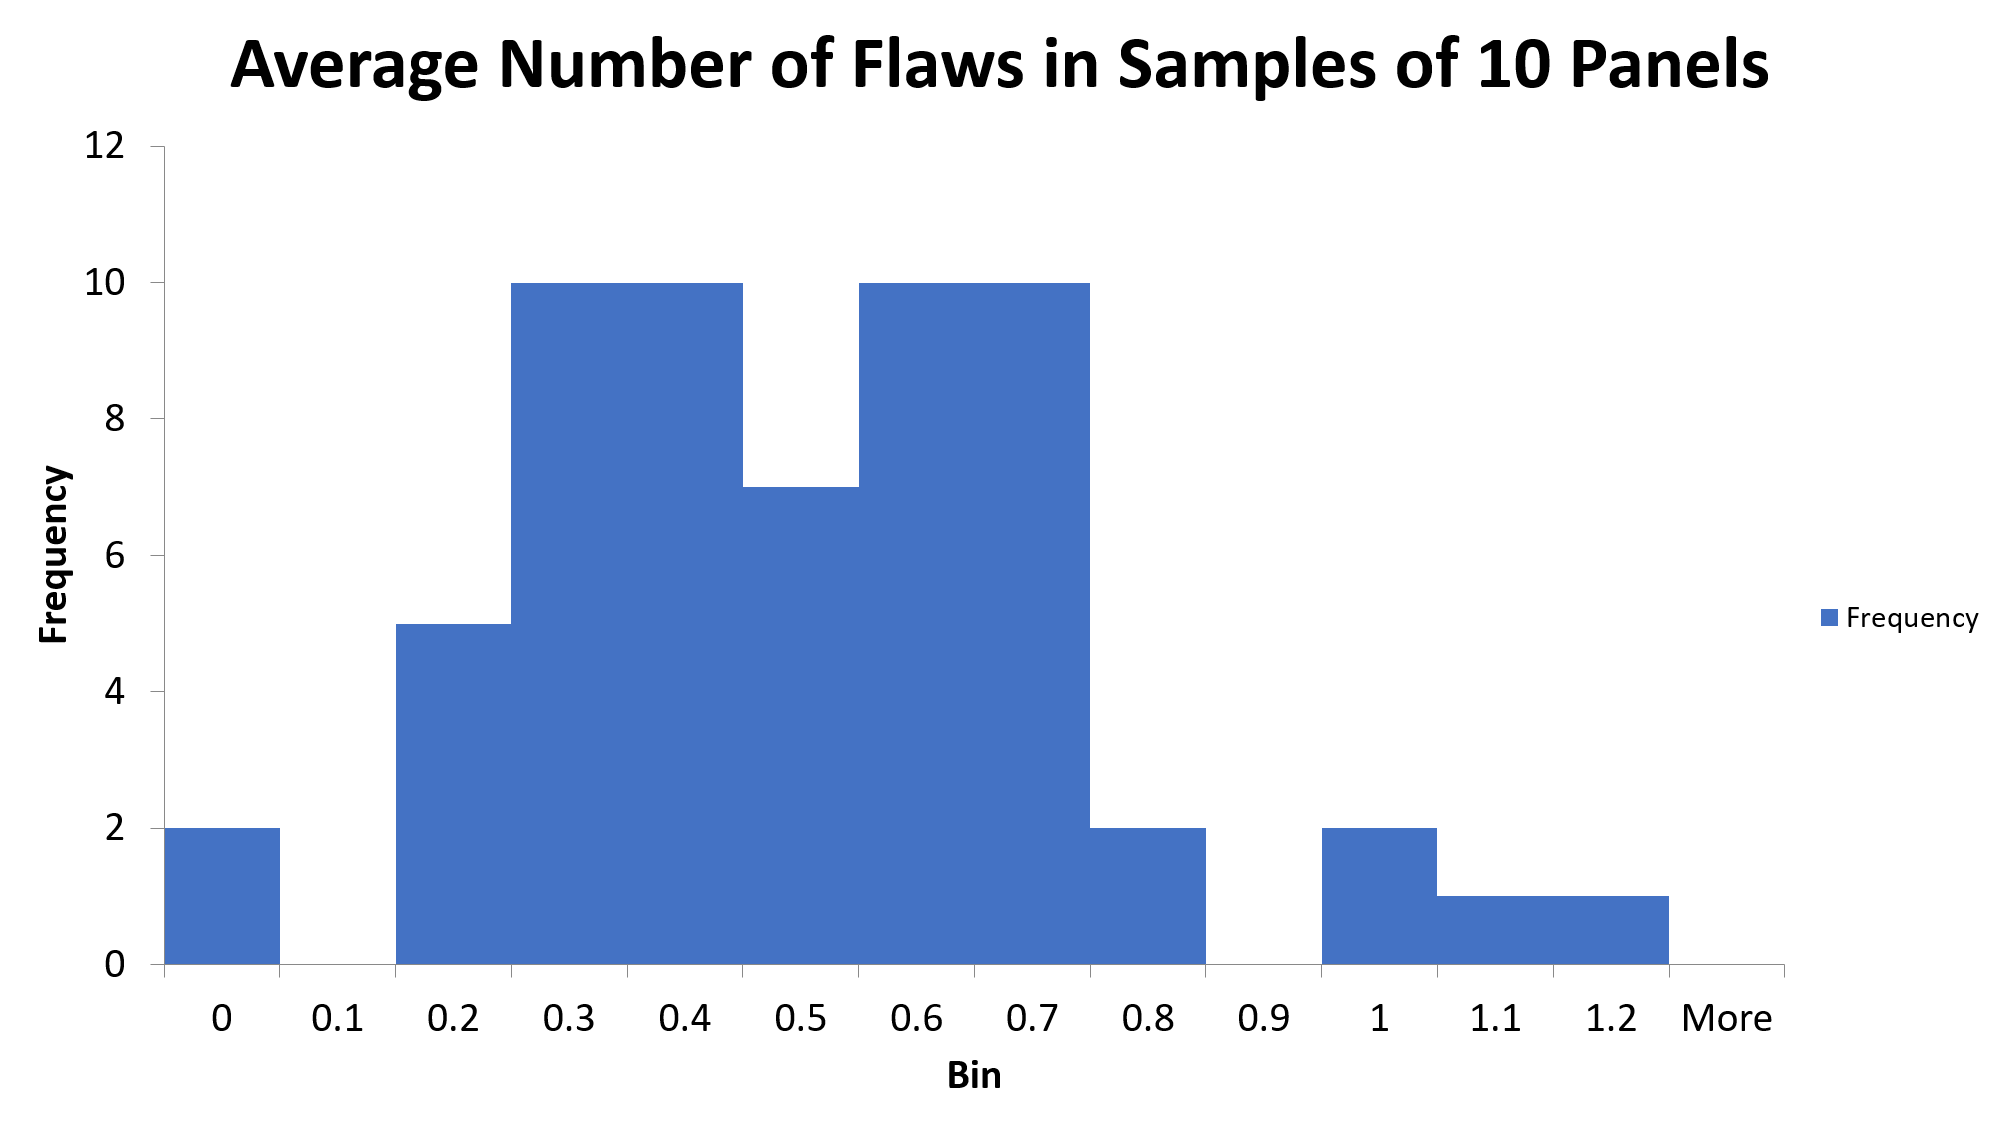
\includegraphics[width=\textwidth]{q4.png}
 \caption{Average number of flaws in samples of 10 panels from 600 plastic panels.}
 \label{4c}
\end{figure}

The histogram above does not seem to resemble a normal distribution. When taking
a step back and looking at the overall shape, it appears to be bimodal with the
first peak being between 0.3-0.4 and the second peak being between 0.6-0.7.

\subsection{}%4d
% Summary statistics calculated automatically.
% Are the predicted values close?
% If they aren't perfect, why not?
From the automatically computed summary statistics in the \textit{Simulation}
worksheet, we find the mean and standard deviation of the average number of
flaws for the 60 samples to be: ($\mu=0.506666667,
 \sigma_{\bar{x}}=0.242771195$). In \ref{3a}, we found the theoretical values to
be ($\lambda=\mu=0.5, \sigma_{\bar{x}}=0.2236$). These values aren't the exact
same, but they are really close. We expected these values to be close, however,
it would be unrealistic for them to be exactly the same, due to the randomness
of the data, and also because we are taking samples from 600 randomly generated
panels while the theoretical value is from taking samples from an infinite
number of panels.

\section{}%5

\subsection{}%5a
% Basically, repeat question 4c, d with n=30
% Redo the random simulation
% When comparing, how does the central limit theorem apply?

\begin{figure}[H]
 \centering
 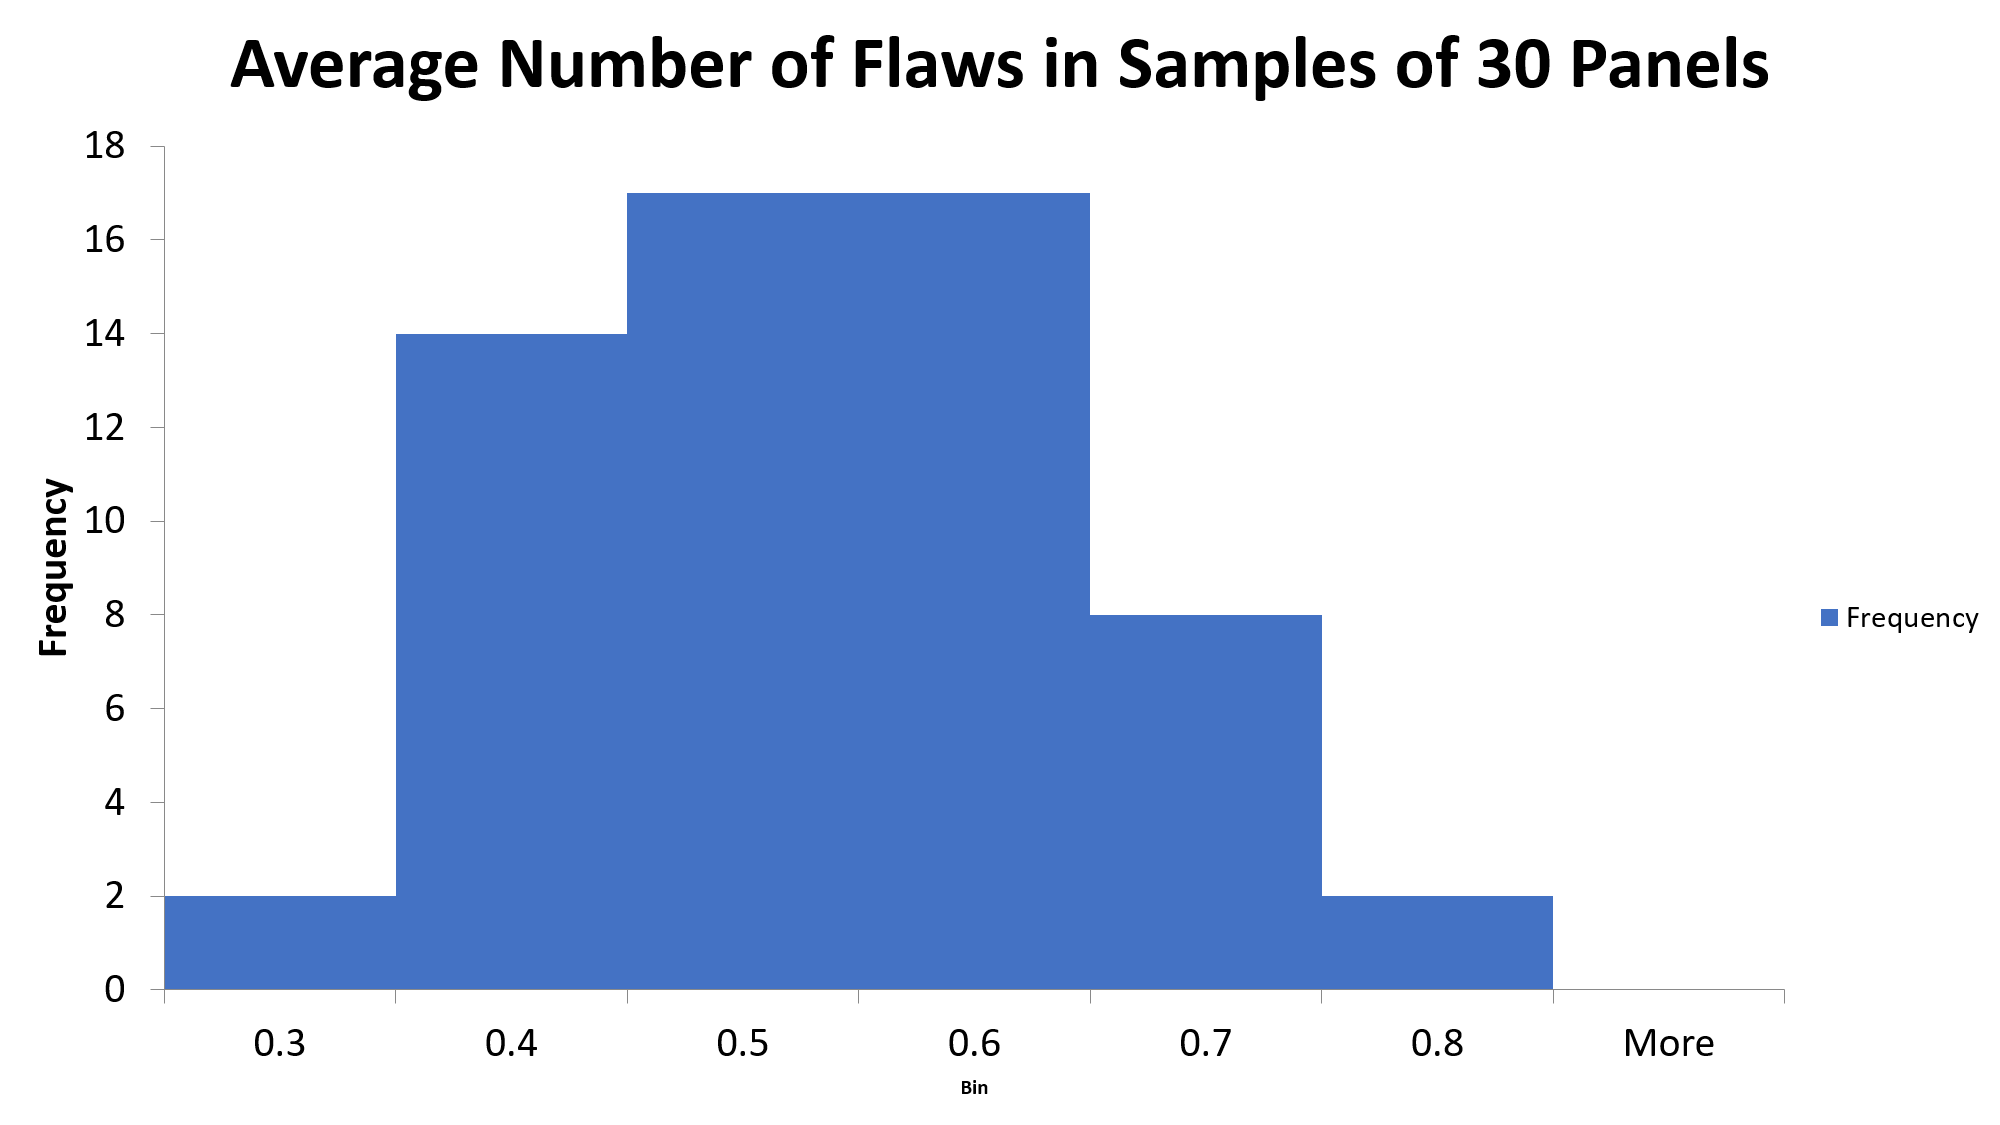
\includegraphics[width=\textwidth]{q5.png}
 \caption{INSERT CAPTION HERE}
 \label{5a}
\end{figure}

\subsection{}%5b
% Why is this estimate better/worse?


\end{document}
